\documentclass[a4paper,12pt]{article}
\usepackage{graphicx}
\usepackage{amsmath, amssymb}
\usepackage{hyperref}
\usepackage{tikz}
\usepackage[backend=biber, style=numeric, citestyle=ieee]{biblatex}

\addbibresource{references.bib}


\title{Centripetal Force: Technical Paper for Activity 3}
\author{Janelle Lastimado \\
John Paul Memoracion \\ 
Nikki Shane Mercado \\
Gian Myrl Renomeron}
\date{February 6, 2025}

\begin{document}

\maketitle

\begin{abstract}

\end{abstract}

\section{Introduction}

\section{Materials and Methodology}


\subsection{Materials}
Below are the list of materials used in the experiment
\begin{itemize}
    \item Pen case
    \item Fishline
    \item Paper clip
    \item Platform balance
    \item Stopwatch
    \item Cork
    \item Set of Masses
\end{itemize}

\subsection{Methodology}
The goal of this experiment is to determine the centripetal force acting on a rotating object. Figure \ref{fig:setup} shows the setup of the experiment.


\paragraph{Procedure}

\begin{figure}[]
    \centering
    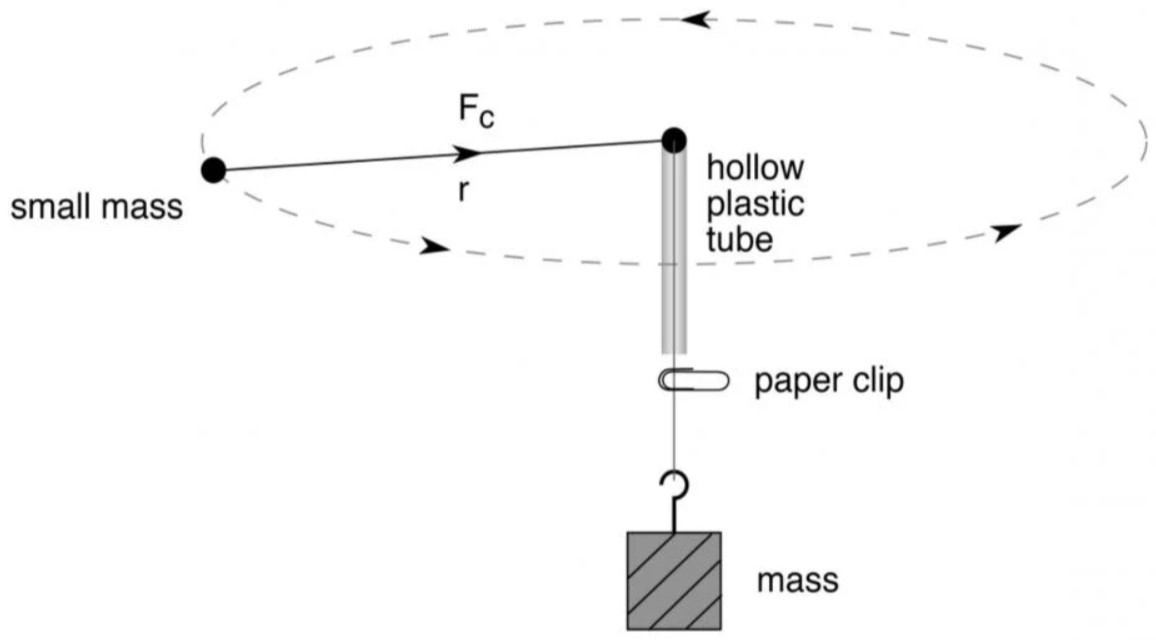
\includegraphics[width=1\textwidth]{experiment_setup.png}
    \caption{Experimental setup}
    \label{fig:setup}
\end{figure}

\begin{enumerate}
    \item Measure the mass of the cork. Hang a 50 g mass on one end of the fishline (this serves as the theoretical value for the centripetal force). Insert the other end into the pen case. The cork must be tied to this end. Support the mass with one hand and hold the pen case in the other.
    \item Fasten a paper clip just below the bottom of the pen case. Whirl the cork by revolving the pen case. Slowly release the 50 g mass and adjust the speed of revolution so that the paper clip stays in place.
    \item Next, grasp the string at the bottom of the pen case to mark the position of the string while the cork is moving. With the string in this position, measure the radius \textbf{r}.
    \item For the same mass change the radius of the rotation first to the smaller value and then to a larger value. Observe the corresponding change to maintain the mass at the stationary position.
\end{enumerate}


\section{Results and Discussion}
Below is the data and result of the experiments. The weighted hanger was used as the force. Marbles were used to increase the weight of the hanger. In Experiment 1, 10 marbles were used in the first trial, 11 were used in the second trial, and 12 were used in the third trial. In Experiment 2, the marbles used in the weighted hanger were constant (10 marbles). The mass was of the truck was increased using marbles and batteries. Each battery weighted 25g and each marble weighted 5g.

\subsection{Experiment 1: Mass constant, Force varies}
\begin{table}[h]
    \centering
    \renewcommand{\arraystretch}{1.2}
    \makebox[\textwidth]{ 
        \begin{tabular}{|c|c|c|c|c|c|c|}
            \hline
            \textbf{Trial} & \textbf{m (kg)} & \textbf{r (m)} & \textbf{Period (s)} & \textbf{$v$ (m/s)} & \textbf{$v^2$ (m/s)} & \textbf{F (N)} \\
            \hline
            1 & 0.033 kg & 0.49 N & 0.32 s & 0.71 m & 14.8 m/s\(^2\) & 13.87 m/s\(^2\) \\
            2 & 0.033 kg & 0.539 N & 0.29 s & 0.71 m & 16.3 m/s\(^2\) & 16.88 m/s\(^2\) \\
            3 & 0.033 kg & 0.588 N & 0.27 s & 0.71 m & 17.8 m/s\(^2\) & 19.47 m/s\(^2\) \\
            \hline
        \end{tabular}
    }
    \caption{Results of the Experiment}
    \label{table:exp}
\end{table}

As one can see in table \ref{table:exp} for the first experiment, constant mass of cart with varying forces were applied on the cart and their acceleration in theory and actual measurement are very clear. From these values acceleration due to increased force is obtained and it does agree with the second law formulated by Newtons as \( F = ma \), with a constant value of mass in that case it will be more or less proportionate to an acceleration. \\

Experimental acceleration values are quite close to the theoretical one, despite some slight differences. These can be caused by the friction from the surface and air friction around the test body, errors in measurement or reaction time to start and stop the stopwatch. Despite such minute differences, the trend clearly shows that acceleration increases with force, as expected by the theory.

\section{Conclusion}

The experiment was successful in testing the Newton's Second Law of Motion. The investigation found that constant mass allows an increase in force resulting in increased acceleration. An increase in mass with constant force leads to reduced acceleration. Following the expected trends as determined by the equation: \( F = ma \), which also corresponds directly to the relationships between force, mass, and acceleration.

\printbibliography

\end{document}
